\subsubsection{Tipos y Caracter\'isticas}
\label{subsubsection:tiposYCaractCubelets}
    % Parrafo 1
    A continuaci\'on mencionaremos los tipos de Cubelets que existen y sus caracter\'isticas, estos fueron extraidos de la p\'agina ofical de los
        cubelets \cite{modrobotics2023}.
    \begin{itemize}
        \begin{minipage}
            {0.5\textwidth}
            \item \textbf{Cubelet de Gr\'afico de barras}: Muestra el valor del bloque en el gr\'afico
                de barras luminoso de 10 segmentos. El valor se adapta de 0 a 255, y se visualiza en 10 
                segmentos de 25.5 cada uno.
        \end{minipage}
        \begin{minipage}
            {0.5\textwidth}
            \centering
            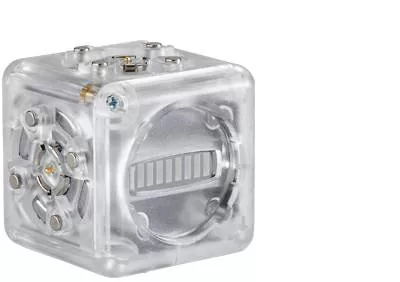
\includegraphics[width=0.5\textwidth]{./images/marco_teorico/cubelets/graficoDeBarras.png}
        \end{minipage}
        \begin{minipage}
            {0.5\textwidth}
            \item \textbf{Cubelet de Bater\'ia}: Da energ\'ia a los Cubelets conectados a \'el. 
                La bater\'ia se recarga a trav\'es de un puerto micro USB.
        \end{minipage}
        \begin{minipage}
            {0.5\textwidth}
            \centering
            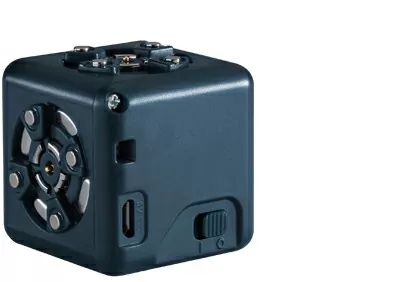
\includegraphics[width=0.5\textwidth]{./images/marco_teorico/cubelets/bateria.png}
        \end{minipage}
        \begin{minipage}
            {0.5\textwidth}
            \item \textbf{Cubelet Bloquedor}: Bloquea el flujo de datos de sus vecinos.
                Permite el paso de energ\'ia pero no de datos.
        \end{minipage}
        \begin{minipage}
            {0.5\textwidth}
            \centering
            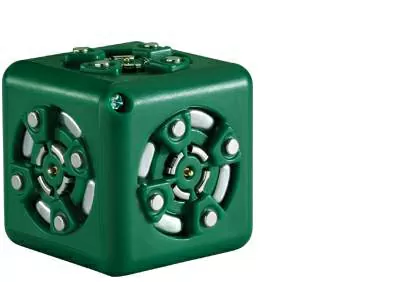
\includegraphics[width=0.5\textwidth]{./images/marco_teorico/cubelets/bloqueador.png}
        \end{minipage}
        \begin{minipage}
            {0.5\textwidth}
            \item \textbf{Cubelet de Bluethooth}: Permite la comunicaci\'on inal\'ambrica entre
                los Cubelets y otros dispositivos. Sin embargo esto solo lo hace para programar el 
                comportamiento de los Cubelets, no para la transmisi\'on de datos.
        \end{minipage}
        \begin{minipage}
            {0.5\textwidth}
            \centering
            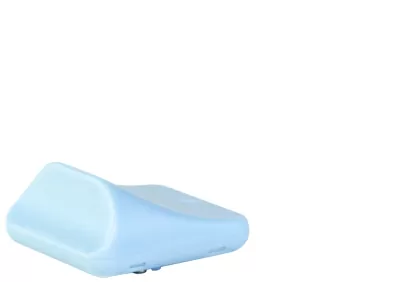
\includegraphics[width=0.5\textwidth]{./images/marco_teorico/cubelets/bluetooth.png}
        \end{minipage}
        \begin{minipage}
            {0.5\textwidth}
            \item \textbf{Cubelet de Sensor de Luz}: Mide la intensidad de la luz en su entorno.
        \end{minipage}
        \begin{minipage}
            {0.5\textwidth}
            \centering
            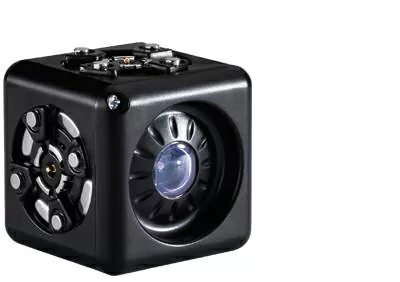
\includegraphics[width=0.5\textwidth]{./images/marco_teorico/cubelets/sensorDeLuz.png}
        \end{minipage}
        \begin{minipage}
            {0.5\textwidth}
            \item \textbf{Cubelet de Distancia}: Mide la distancia a un objeto en su entorno.
        \end{minipage}
        \begin{minipage}
            {0.5\textwidth}
            \centering
            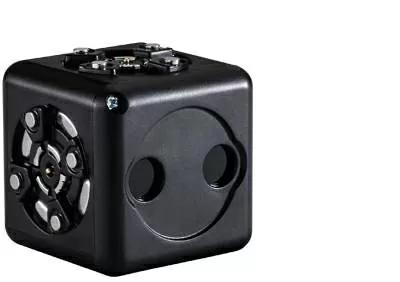
\includegraphics[width=0.5\textwidth]{./images/marco_teorico/cubelets/sensorDeDistancia.png}
        \end{minipage}
        \begin{minipage}
            {0.5\textwidth}
            \item \textbf{Cubelet de Temperatura}: Mide la temperatura en su entorno.
        \end{minipage}
        \begin{minipage}
            {0.5\textwidth}
            \centering
            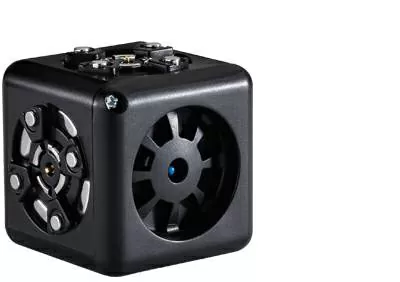
\includegraphics[width=0.5\textwidth]{./images/marco_teorico/cubelets/sensorDeTemperatura.png}
        \end{minipage}
        \begin{minipage}
            {0.5\textwidth}
            \item \textbf{Cubelet de Movimiento}: Es un cubelet que con 2 llantas y un motor, 
                permite que el robot se mueva.
        \end{minipage}
        \begin{minipage}
            {0.5\textwidth}
            \centering
            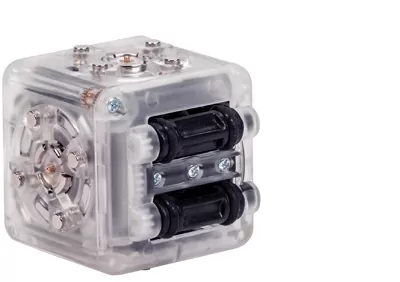
\includegraphics[width=0.5\textwidth]{./images/marco_teorico/cubelets/movimiento.png}
        \end{minipage}
        \begin{minipage}
            {0.5\textwidth}
            \item \textbf{Cubelet de Luz}: Emite luz con un led blanco y dependiendo del valor que 
                reciba, la intensidad de la luz variar\'a.
        \end{minipage}
        \begin{minipage}
            {0.5\textwidth}
            \centering
            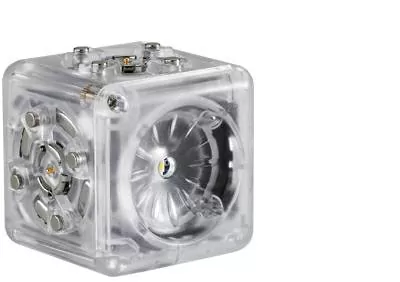
\includegraphics[width=0.5\textwidth]{./images/marco_teorico/cubelets/luz.png}
        \end{minipage}
        \begin{minipage}
            {0.5\textwidth}
            \item \textbf{Cubelet de Inversor}: Invierte el valor que recibe, es decir, si recibe un 0,
                emitir\'a un 255 y viceversa.
        \end{minipage}
        \begin{minipage}
            {0.5\textwidth}
            \centering
            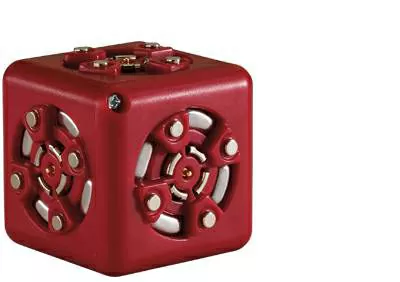
\includegraphics[width=0.5\textwidth]{./images/marco_teorico/cubelets/inversor.png}
        \end{minipage}
        \begin{minipage}
            {0.5\textwidth}
            \item \textbf{Cubelet de Perilla}: Permite ajustar el valor que recibe, es decir, si recibe
                un 0, emitir\'a un 0, si recibe un 255, emitir\'a un 255 y si recibe un valor intermedio,
                emitir\'a un valor intermedio.
        \end{minipage}
        \begin{minipage}
            {0.5\textwidth}
            \centering
            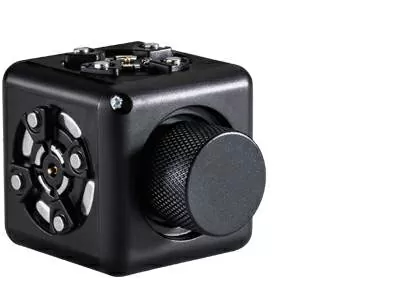
\includegraphics[width=0.5\textwidth]{./images/marco_teorico/cubelets/perilla.png}
        \end{minipage}
        \begin{minipage}
            {0.5\textwidth}
            \item \textbf{Cubelet de M\'aximo}: Emite el valor m\'as alto que recibe.
        \end{minipage}
        \begin{minipage}
            {0.5\textwidth}
            \centering
            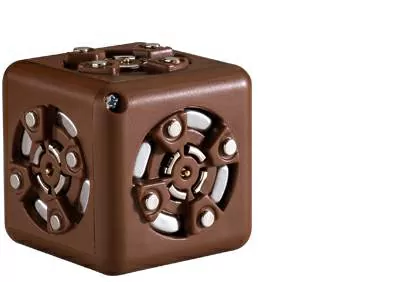
\includegraphics[width=0.5\textwidth]{./images/marco_teorico/cubelets/maximo.png}
        \end{minipage}
        \begin{minipage}
            {0.5\textwidth}
            \item \textbf{Cubelet de M\'inimo}: Emite el valor m\'as bajo que recibe.
        \end{minipage}
        \begin{minipage}
            {0.5\textwidth}
            \centering
            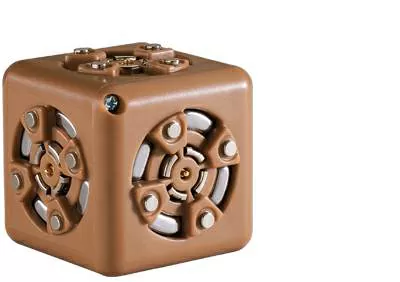
\includegraphics[width=0.5\textwidth]{./images/marco_teorico/cubelets/minimo.png}
        \end{minipage}
        \begin{minipage}
            {0.5\textwidth}
            \item \textbf{Cubelet Pasivo}: No tiene ninguna funci\'on, solo sirve para conectar los 
                Cubelets entre s\'i.
        \end{minipage}
        \begin{minipage}
            {0.5\textwidth}
            \centering
            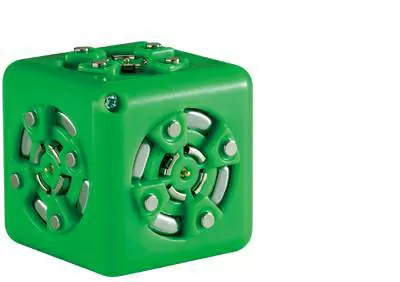
\includegraphics[width=0.5\textwidth]{./images/marco_teorico/cubelets/pasivo.png}
        \end{minipage}
        \begin{minipage}
            {0.5\textwidth}
            \item \textbf{Cubelet de Buzzer}: Emite un sonido con una frecuencia dependiendo del valor
                que recibe.
        \end{minipage}
        \begin{minipage}
            {0.5\textwidth}
            \centering
            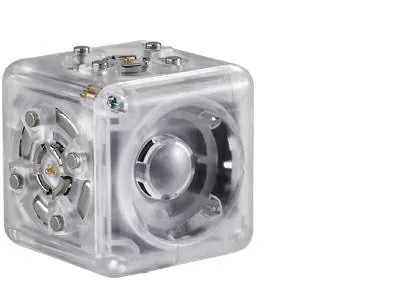
\includegraphics[width=0.5\textwidth]{./images/marco_teorico/cubelets/buzzer.png}
        \end{minipage}
        \begin{minipage}
            {0.5\textwidth}
            \item \textbf{Cubelet Rotativo}: Con un motor gira dependiendo del valor que recibe.
        \end{minipage}
        \begin{minipage}
            {0.5\textwidth}
            \centering
            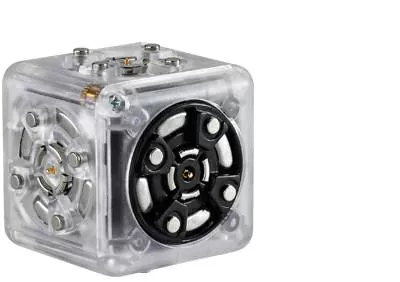
\includegraphics[width=0.5\textwidth]{./images/marco_teorico/cubelets/rotativo.png}
        \end{minipage}
        \begin{minipage}
            {0.5\textwidth}
            \item \textbf{Cubelet Umbral}:  El Threshold Cubelet es un THINK Cubelet con una perilla para alterar 
                el comportamiento de tus robots. Emitir\'a un valor de cero hasta que sus entradas superen el umbral establecido 
                por la perilla. Por encima de este umbral, los datos fluir\'an normalmente.
        \end{minipage}
        \begin{minipage}
            {0.5\textwidth}
            \centering
            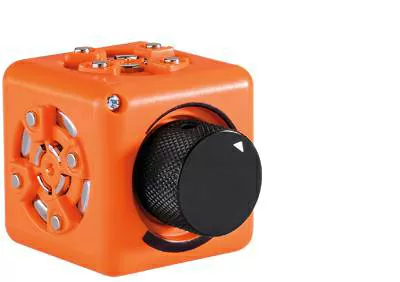
\includegraphics[width=0.5\textwidth]{./images/marco_teorico/cubelets/umbral.png}
        \end{minipage}
    \end{itemize}